


% Header, overrides base

    % Make sure that the sphinx doc style knows who it inherits from.
    \def\sphinxdocclass{article}

    % Declare the document class
    \documentclass[letterpaper,10pt,english]{/usr/share/sphinx/texinputs/sphinxhowto}

    % Imports
    \usepackage[utf8]{inputenc}
    \DeclareUnicodeCharacter{00A0}{\\nobreakspace}
    \usepackage[T1]{fontenc}
    \usepackage{babel}
    \usepackage{times}
    \usepackage{import}
    \usepackage[Bjarne]{/usr/share/sphinx/texinputs/fncychap}
    \usepackage{longtable}
    \usepackage{/usr/share/sphinx/texinputs/sphinx}
    \usepackage{multirow}

    \usepackage{amsmath}
    \usepackage{amssymb}
    \usepackage{ucs}
    \usepackage{enumerate}

    % Used to make the Input/Output rules follow around the contents.
    \usepackage{needspace}

    % Pygments requirements
    \usepackage{fancyvrb}
    \usepackage{color}
    % ansi colors additions
    \definecolor{darkgreen}{rgb}{.12,.54,.11}
    \definecolor{lightgray}{gray}{.95}
    \definecolor{brown}{rgb}{0.54,0.27,0.07}
    \definecolor{purple}{rgb}{0.5,0.0,0.5}
    \definecolor{darkgray}{gray}{0.25}
    \definecolor{lightred}{rgb}{1.0,0.39,0.28}
    \definecolor{lightgreen}{rgb}{0.48,0.99,0.0}
    \definecolor{lightblue}{rgb}{0.53,0.81,0.92}
    \definecolor{lightpurple}{rgb}{0.87,0.63,0.87}
    \definecolor{lightcyan}{rgb}{0.5,1.0,0.83}

    % Needed to box output/input
    \usepackage{tikz}
        \usetikzlibrary{calc,arrows,shadows}
    \usepackage[framemethod=tikz]{mdframed}

    \usepackage{alltt}

    % Used to load and display graphics
    \usepackage{graphicx}
    \graphicspath{ {figs/} }
    \usepackage[Export]{adjustbox} % To resize

    % used so that images for notebooks which have spaces in the name can still be included
    \usepackage{grffile}


    % For formatting output while also word wrapping.
    \usepackage{listings}
    \lstset{breaklines=true}
    \lstset{basicstyle=\small\ttfamily}
    \def\smaller{\fontsize{9.5pt}{9.5pt}\selectfont}

    %Pygments definitions
    
\makeatletter
\def\PY@reset{\let\PY@it=\relax \let\PY@bf=\relax%
    \let\PY@ul=\relax \let\PY@tc=\relax%
    \let\PY@bc=\relax \let\PY@ff=\relax}
\def\PY@tok#1{\csname PY@tok@#1\endcsname}
\def\PY@toks#1+{\ifx\relax#1\empty\else%
    \PY@tok{#1}\expandafter\PY@toks\fi}
\def\PY@do#1{\PY@bc{\PY@tc{\PY@ul{%
    \PY@it{\PY@bf{\PY@ff{#1}}}}}}}
\def\PY#1#2{\PY@reset\PY@toks#1+\relax+\PY@do{#2}}

\expandafter\def\csname PY@tok@gd\endcsname{\def\PY@tc##1{\textcolor[rgb]{0.63,0.00,0.00}{##1}}}
\expandafter\def\csname PY@tok@gu\endcsname{\let\PY@bf=\textbf\def\PY@tc##1{\textcolor[rgb]{0.50,0.00,0.50}{##1}}}
\expandafter\def\csname PY@tok@gt\endcsname{\def\PY@tc##1{\textcolor[rgb]{0.00,0.27,0.87}{##1}}}
\expandafter\def\csname PY@tok@gs\endcsname{\let\PY@bf=\textbf}
\expandafter\def\csname PY@tok@gr\endcsname{\def\PY@tc##1{\textcolor[rgb]{1.00,0.00,0.00}{##1}}}
\expandafter\def\csname PY@tok@cm\endcsname{\let\PY@it=\textit\def\PY@tc##1{\textcolor[rgb]{0.25,0.50,0.50}{##1}}}
\expandafter\def\csname PY@tok@vg\endcsname{\def\PY@tc##1{\textcolor[rgb]{0.10,0.09,0.49}{##1}}}
\expandafter\def\csname PY@tok@m\endcsname{\def\PY@tc##1{\textcolor[rgb]{0.40,0.40,0.40}{##1}}}
\expandafter\def\csname PY@tok@mh\endcsname{\def\PY@tc##1{\textcolor[rgb]{0.40,0.40,0.40}{##1}}}
\expandafter\def\csname PY@tok@go\endcsname{\def\PY@tc##1{\textcolor[rgb]{0.53,0.53,0.53}{##1}}}
\expandafter\def\csname PY@tok@ge\endcsname{\let\PY@it=\textit}
\expandafter\def\csname PY@tok@vc\endcsname{\def\PY@tc##1{\textcolor[rgb]{0.10,0.09,0.49}{##1}}}
\expandafter\def\csname PY@tok@il\endcsname{\def\PY@tc##1{\textcolor[rgb]{0.40,0.40,0.40}{##1}}}
\expandafter\def\csname PY@tok@cs\endcsname{\let\PY@it=\textit\def\PY@tc##1{\textcolor[rgb]{0.25,0.50,0.50}{##1}}}
\expandafter\def\csname PY@tok@cp\endcsname{\def\PY@tc##1{\textcolor[rgb]{0.74,0.48,0.00}{##1}}}
\expandafter\def\csname PY@tok@gi\endcsname{\def\PY@tc##1{\textcolor[rgb]{0.00,0.63,0.00}{##1}}}
\expandafter\def\csname PY@tok@gh\endcsname{\let\PY@bf=\textbf\def\PY@tc##1{\textcolor[rgb]{0.00,0.00,0.50}{##1}}}
\expandafter\def\csname PY@tok@ni\endcsname{\let\PY@bf=\textbf\def\PY@tc##1{\textcolor[rgb]{0.60,0.60,0.60}{##1}}}
\expandafter\def\csname PY@tok@nl\endcsname{\def\PY@tc##1{\textcolor[rgb]{0.63,0.63,0.00}{##1}}}
\expandafter\def\csname PY@tok@nn\endcsname{\let\PY@bf=\textbf\def\PY@tc##1{\textcolor[rgb]{0.00,0.00,1.00}{##1}}}
\expandafter\def\csname PY@tok@no\endcsname{\def\PY@tc##1{\textcolor[rgb]{0.53,0.00,0.00}{##1}}}
\expandafter\def\csname PY@tok@na\endcsname{\def\PY@tc##1{\textcolor[rgb]{0.49,0.56,0.16}{##1}}}
\expandafter\def\csname PY@tok@nb\endcsname{\def\PY@tc##1{\textcolor[rgb]{0.00,0.50,0.00}{##1}}}
\expandafter\def\csname PY@tok@nc\endcsname{\let\PY@bf=\textbf\def\PY@tc##1{\textcolor[rgb]{0.00,0.00,1.00}{##1}}}
\expandafter\def\csname PY@tok@nd\endcsname{\def\PY@tc##1{\textcolor[rgb]{0.67,0.13,1.00}{##1}}}
\expandafter\def\csname PY@tok@ne\endcsname{\let\PY@bf=\textbf\def\PY@tc##1{\textcolor[rgb]{0.82,0.25,0.23}{##1}}}
\expandafter\def\csname PY@tok@nf\endcsname{\def\PY@tc##1{\textcolor[rgb]{0.00,0.00,1.00}{##1}}}
\expandafter\def\csname PY@tok@si\endcsname{\let\PY@bf=\textbf\def\PY@tc##1{\textcolor[rgb]{0.73,0.40,0.53}{##1}}}
\expandafter\def\csname PY@tok@s2\endcsname{\def\PY@tc##1{\textcolor[rgb]{0.73,0.13,0.13}{##1}}}
\expandafter\def\csname PY@tok@vi\endcsname{\def\PY@tc##1{\textcolor[rgb]{0.10,0.09,0.49}{##1}}}
\expandafter\def\csname PY@tok@nt\endcsname{\let\PY@bf=\textbf\def\PY@tc##1{\textcolor[rgb]{0.00,0.50,0.00}{##1}}}
\expandafter\def\csname PY@tok@nv\endcsname{\def\PY@tc##1{\textcolor[rgb]{0.10,0.09,0.49}{##1}}}
\expandafter\def\csname PY@tok@s1\endcsname{\def\PY@tc##1{\textcolor[rgb]{0.73,0.13,0.13}{##1}}}
\expandafter\def\csname PY@tok@sh\endcsname{\def\PY@tc##1{\textcolor[rgb]{0.73,0.13,0.13}{##1}}}
\expandafter\def\csname PY@tok@sc\endcsname{\def\PY@tc##1{\textcolor[rgb]{0.73,0.13,0.13}{##1}}}
\expandafter\def\csname PY@tok@sx\endcsname{\def\PY@tc##1{\textcolor[rgb]{0.00,0.50,0.00}{##1}}}
\expandafter\def\csname PY@tok@bp\endcsname{\def\PY@tc##1{\textcolor[rgb]{0.00,0.50,0.00}{##1}}}
\expandafter\def\csname PY@tok@c1\endcsname{\let\PY@it=\textit\def\PY@tc##1{\textcolor[rgb]{0.25,0.50,0.50}{##1}}}
\expandafter\def\csname PY@tok@kc\endcsname{\let\PY@bf=\textbf\def\PY@tc##1{\textcolor[rgb]{0.00,0.50,0.00}{##1}}}
\expandafter\def\csname PY@tok@c\endcsname{\let\PY@it=\textit\def\PY@tc##1{\textcolor[rgb]{0.25,0.50,0.50}{##1}}}
\expandafter\def\csname PY@tok@mf\endcsname{\def\PY@tc##1{\textcolor[rgb]{0.40,0.40,0.40}{##1}}}
\expandafter\def\csname PY@tok@err\endcsname{\def\PY@bc##1{\setlength{\fboxsep}{0pt}\fcolorbox[rgb]{1.00,0.00,0.00}{1,1,1}{\strut ##1}}}
\expandafter\def\csname PY@tok@kd\endcsname{\let\PY@bf=\textbf\def\PY@tc##1{\textcolor[rgb]{0.00,0.50,0.00}{##1}}}
\expandafter\def\csname PY@tok@ss\endcsname{\def\PY@tc##1{\textcolor[rgb]{0.10,0.09,0.49}{##1}}}
\expandafter\def\csname PY@tok@sr\endcsname{\def\PY@tc##1{\textcolor[rgb]{0.73,0.40,0.53}{##1}}}
\expandafter\def\csname PY@tok@mo\endcsname{\def\PY@tc##1{\textcolor[rgb]{0.40,0.40,0.40}{##1}}}
\expandafter\def\csname PY@tok@kn\endcsname{\let\PY@bf=\textbf\def\PY@tc##1{\textcolor[rgb]{0.00,0.50,0.00}{##1}}}
\expandafter\def\csname PY@tok@mi\endcsname{\def\PY@tc##1{\textcolor[rgb]{0.40,0.40,0.40}{##1}}}
\expandafter\def\csname PY@tok@gp\endcsname{\let\PY@bf=\textbf\def\PY@tc##1{\textcolor[rgb]{0.00,0.00,0.50}{##1}}}
\expandafter\def\csname PY@tok@o\endcsname{\def\PY@tc##1{\textcolor[rgb]{0.40,0.40,0.40}{##1}}}
\expandafter\def\csname PY@tok@kr\endcsname{\let\PY@bf=\textbf\def\PY@tc##1{\textcolor[rgb]{0.00,0.50,0.00}{##1}}}
\expandafter\def\csname PY@tok@s\endcsname{\def\PY@tc##1{\textcolor[rgb]{0.73,0.13,0.13}{##1}}}
\expandafter\def\csname PY@tok@kp\endcsname{\def\PY@tc##1{\textcolor[rgb]{0.00,0.50,0.00}{##1}}}
\expandafter\def\csname PY@tok@w\endcsname{\def\PY@tc##1{\textcolor[rgb]{0.73,0.73,0.73}{##1}}}
\expandafter\def\csname PY@tok@kt\endcsname{\def\PY@tc##1{\textcolor[rgb]{0.69,0.00,0.25}{##1}}}
\expandafter\def\csname PY@tok@ow\endcsname{\let\PY@bf=\textbf\def\PY@tc##1{\textcolor[rgb]{0.67,0.13,1.00}{##1}}}
\expandafter\def\csname PY@tok@sb\endcsname{\def\PY@tc##1{\textcolor[rgb]{0.73,0.13,0.13}{##1}}}
\expandafter\def\csname PY@tok@k\endcsname{\let\PY@bf=\textbf\def\PY@tc##1{\textcolor[rgb]{0.00,0.50,0.00}{##1}}}
\expandafter\def\csname PY@tok@se\endcsname{\let\PY@bf=\textbf\def\PY@tc##1{\textcolor[rgb]{0.73,0.40,0.13}{##1}}}
\expandafter\def\csname PY@tok@sd\endcsname{\let\PY@it=\textit\def\PY@tc##1{\textcolor[rgb]{0.73,0.13,0.13}{##1}}}

\def\PYZbs{\char`\\}
\def\PYZus{\char`\_}
\def\PYZob{\char`\{}
\def\PYZcb{\char`\}}
\def\PYZca{\char`\^}
\def\PYZam{\char`\&}
\def\PYZlt{\char`\<}
\def\PYZgt{\char`\>}
\def\PYZsh{\char`\#}
\def\PYZpc{\char`\%}
\def\PYZdl{\char`\$}
\def\PYZhy{\char`\-}
\def\PYZsq{\char`\'}
\def\PYZdq{\char`\"}
\def\PYZti{\char`\~}
% for compatibility with earlier versions
\def\PYZat{@}
\def\PYZlb{[}
\def\PYZrb{]}
\makeatother


    %Set pygments styles if needed...
    
        \definecolor{nbframe-border}{rgb}{0.867,0.867,0.867}
        \definecolor{nbframe-bg}{rgb}{0.969,0.969,0.969}
        \definecolor{nbframe-in-prompt}{rgb}{0.0,0.0,0.502}
        \definecolor{nbframe-out-prompt}{rgb}{0.545,0.0,0.0}

        \newenvironment{ColorVerbatim}
        {\begin{mdframed}[%
            roundcorner=1.0pt, %
            backgroundcolor=nbframe-bg, %
            userdefinedwidth=1\linewidth, %
            leftmargin=0.1\linewidth, %
            innerleftmargin=0pt, %
            innerrightmargin=0pt, %
            linecolor=nbframe-border, %
            linewidth=1pt, %
            usetwoside=false, %
            everyline=true, %
            innerlinewidth=3pt, %
            innerlinecolor=nbframe-bg, %
            middlelinewidth=1pt, %
            middlelinecolor=nbframe-bg, %
            outerlinewidth=0.5pt, %
            outerlinecolor=nbframe-border, %
            needspace=0pt
        ]}
        {\end{mdframed}}
        
        \newenvironment{InvisibleVerbatim}
        {\begin{mdframed}[leftmargin=0.1\linewidth,innerleftmargin=3pt,innerrightmargin=3pt, userdefinedwidth=1\linewidth, linewidth=0pt, linecolor=white, usetwoside=false]}
        {\end{mdframed}}

        \renewenvironment{Verbatim}[1][\unskip]
        {\begin{alltt}\smaller}
        {\end{alltt}}
    

    % Help prevent overflowing lines due to urls and other hard-to-break 
    % entities.  This doesn't catch everything...
    \sloppy

    % Document level variables
    \title{Physics IA - Data Analysis}
    \date{February 29, 2016}
    \release{}
    \author{Unknown Author}
    \renewcommand{\releasename}{}

    % TODO: Add option for the user to specify a logo for his/her export.
    \newcommand{\sphinxlogo}{}

    % Make the index page of the document.
    \makeindex

    % Import sphinx document type specifics.
     


% Body

    % Start of the document
    \begin{document}

        
            \maketitle
        

        


        
        

    % Make sure that atleast 4 lines are below the HR
    \needspace{4\baselineskip}

    
        \vspace{6pt}
        \makebox[0.1\linewidth]{\smaller\hfill\tt\color{nbframe-in-prompt}In\hspace{4pt}{[}113{]}:\hspace{4pt}}\\*
        \vspace{-2.65\baselineskip}
        \begin{ColorVerbatim}
            \vspace{-0.7\baselineskip}
            \begin{Verbatim}[commandchars=\\\{\}]
\PY{k+kn}{import} \PY{n+nn}{math}
\PY{k+kn}{import} \PY{n+nn}{matplotlib} \PY{k+kn}{as} \PY{n+nn}{mpl}
\PY{c}{\PYZsh{} mpl.use(\PYZsq{}pgf\PYZsq{})}
\PY{k+kn}{import} \PY{n+nn}{matplotlib.cm} \PY{k+kn}{as} \PY{n+nn}{cm}
\PY{k+kn}{import} \PY{n+nn}{matplotlib.pyplot} \PY{k+kn}{as} \PY{n+nn}{plt}
\PY{k+kn}{import} \PY{n+nn}{numpy} \PY{k+kn}{as} \PY{n+nn}{np}
\PY{k+kn}{import} \PY{n+nn}{pandas} \PY{k+kn}{as} \PY{n+nn}{pd}

\PY{k+kn}{from} \PY{n+nn}{scipy} \PY{k+kn}{import} \PY{n}{stats}
\PY{k+kn}{from} \PY{n+nn}{matplotlib} \PY{k+kn}{import} \PY{n}{rc}

\PY{o}{\PYZpc{}}\PY{k}{matplotlib} \PY{n}{inline}

\PY{k}{print} \PY{n}{plt}\PY{o}{.}\PY{n}{style}\PY{o}{.}\PY{n}{available}
\PY{c}{\PYZsh{} plt.style.use(\PYZsq{}classic\PYZsq{})}
\end{Verbatim}

            
                \vspace{-0.2\baselineskip}
            
        \end{ColorVerbatim}
    

    

        % If the first block is an image, minipage the image.  Else
        % request a certain amount of space for the input text.
        \needspace{4\baselineskip}
        
        

            % Add document contents.
            
                \begin{InvisibleVerbatim}
                \vspace{-0.5\baselineskip}
\begin{alltt}[u'seaborn-darkgrid', u'seaborn-notebook', u'classic', u'seaborn-
ticks', u'grayscale', u'bmh', u'seaborn-talk', u'dark\_background',
u'ggplot', u'fivethirtyeight', u'seaborn-colorblind', u'seaborn-deep',
u'seaborn-whitegrid', u'seaborn-bright', u'seaborn-poster', u'seaborn-
muted', u'seaborn-paper', u'seaborn-white', u'seaborn-pastel', u
'seaborn-dark', u'seaborn-dark-palette']
\end{alltt}

            \end{InvisibleVerbatim}
            
        
    


    % Make sure that atleast 4 lines are below the HR
    \needspace{4\baselineskip}

    
        \vspace{6pt}
        \makebox[0.1\linewidth]{\smaller\hfill\tt\color{nbframe-in-prompt}In\hspace{4pt}{[}114{]}:\hspace{4pt}}\\*
        \vspace{-2.65\baselineskip}
        \begin{ColorVerbatim}
            \vspace{-0.7\baselineskip}
            \begin{Verbatim}[commandchars=\\\{\}]
\PY{c}{\PYZsh{}\PYZsh{} Change default plot style}
\PY{n}{def\PYZus{}style} \PY{o}{=} \PY{l+s}{\PYZsq{}}\PY{l+s}{bmh}\PY{l+s}{\PYZsq{}}
\PY{n}{plt}\PY{o}{.}\PY{n}{style}\PY{o}{.}\PY{n}{use}\PY{p}{(}\PY{n}{def\PYZus{}style}\PY{p}{)}
\PY{c}{\PYZsh{} plt.style.use(\PYZsq{}grayscale\PYZsq{})}
\PY{n}{fig\PYZus{}scl} \PY{o}{=} \PY{l+m+mi}{3}

\PY{k}{def} \PY{n+nf}{figsize}\PY{p}{(}\PY{n}{scale}\PY{p}{,} \PY{n}{height\PYZus{}ratio}\PY{o}{=}\PY{p}{(}\PY{n}{np}\PY{o}{.}\PY{n}{sqrt}\PY{p}{(}\PY{l+m+mf}{5.0}\PY{p}{)}\PY{o}{\PYZhy{}}\PY{l+m+mf}{1.0}\PY{p}{)}\PY{o}{/}\PY{l+m+mf}{2.0}\PY{p}{)}\PY{p}{:}
    \PY{c}{\PYZsh{} got after running \PYZbs{}the\PYZbs{}textwidth}
    \PY{n}{fig\PYZus{}width\PYZus{}pt} \PY{o}{=} \PY{l+m+mf}{345.000}
    
    \PY{n}{inches\PYZus{}per\PYZus{}pt} \PY{o}{=} \PY{l+m+mf}{1.0}\PY{o}{/}\PY{l+m+mf}{72.0}
    
    \PY{n}{fig\PYZus{}width} \PY{o}{=} \PY{n}{fig\PYZus{}width\PYZus{}pt}\PY{o}{*}\PY{n}{inches\PYZus{}per\PYZus{}pt}\PY{o}{*}\PY{n}{scale}
    \PY{n}{fig\PYZus{}height} \PY{o}{=} \PY{n}{fig\PYZus{}width}\PY{o}{*}\PY{n}{height\PYZus{}ratio}
    \PY{n}{fig\PYZus{}size} \PY{o}{=} \PY{p}{(}\PY{n}{fig\PYZus{}width}\PY{p}{,}\PY{n}{fig\PYZus{}height}\PY{p}{)}
    
    \PY{k}{return} \PY{n}{fig\PYZus{}size}

\PY{k}{def} \PY{n+nf}{setup\PYZus{}tex}\PY{p}{(}\PY{p}{)}\PY{p}{:}
    \PY{l+s+sd}{\PYZdq{}\PYZdq{}\PYZdq{}}
\PY{l+s+sd}{    formats the plots for production with latex}
\PY{l+s+sd}{    \PYZdq{}\PYZdq{}\PYZdq{}}
    \PY{n}{pgf\PYZus{}with\PYZus{}latex} \PY{o}{=} \PY{p}{\PYZob{}}
        \PY{l+s}{\PYZdq{}}\PY{l+s}{pgf.texsystem}\PY{l+s}{\PYZdq{}}\PY{p}{:} \PY{l+s}{\PYZdq{}}\PY{l+s}{pdflatex}\PY{l+s}{\PYZdq{}}\PY{p}{,}
        \PY{l+s}{\PYZdq{}}\PY{l+s}{text.usetex}\PY{l+s}{\PYZdq{}}\PY{p}{:} \PY{n+nb+bp}{True}\PY{p}{,}
        \PY{l+s}{\PYZdq{}}\PY{l+s}{font.family}\PY{l+s}{\PYZdq{}}\PY{p}{:} \PY{l+s}{\PYZdq{}}\PY{l+s}{serif}\PY{l+s}{\PYZdq{}}\PY{p}{,}
        \PY{l+s}{\PYZdq{}}\PY{l+s}{font.serif}\PY{l+s}{\PYZdq{}}\PY{p}{:} \PY{p}{[}\PY{l+s}{\PYZdq{}}\PY{l+s}{palatino}\PY{l+s}{\PYZdq{}}\PY{p}{]}\PY{p}{,}
        \PY{l+s}{\PYZdq{}}\PY{l+s}{font.sans\PYZhy{}serif}\PY{l+s}{\PYZdq{}}\PY{p}{:} \PY{p}{[}\PY{p}{]}\PY{p}{,}
        \PY{l+s}{\PYZdq{}}\PY{l+s}{font.monospace}\PY{l+s}{\PYZdq{}}\PY{p}{:} \PY{p}{[}\PY{p}{]}\PY{p}{,}
        \PY{l+s}{\PYZdq{}}\PY{l+s}{axes.labelsize}\PY{l+s}{\PYZdq{}}\PY{p}{:} \PY{l+m+mi}{10}\PY{p}{,}
        \PY{l+s}{\PYZdq{}}\PY{l+s}{text.fontsize}\PY{l+s}{\PYZdq{}}\PY{p}{:} \PY{l+m+mi}{10}\PY{p}{,}
        \PY{l+s}{\PYZdq{}}\PY{l+s}{legend.fontsize}\PY{l+s}{\PYZdq{}}\PY{p}{:} \PY{l+m+mi}{8}\PY{p}{,}
        \PY{l+s}{\PYZdq{}}\PY{l+s}{xtick.labelsize}\PY{l+s}{\PYZdq{}}\PY{p}{:} \PY{l+m+mi}{8}\PY{p}{,}
        \PY{l+s}{\PYZdq{}}\PY{l+s}{ytick.labelsize}\PY{l+s}{\PYZdq{}}\PY{p}{:} \PY{l+m+mi}{8}\PY{p}{,}
        \PY{l+s}{\PYZdq{}}\PY{l+s}{figure.figsize}\PY{l+s}{\PYZdq{}}\PY{p}{:} \PY{n}{figsize}\PY{p}{(}\PY{l+m+mi}{1}\PY{p}{)}
    \PY{p}{\PYZcb{}}
    \PY{n}{mpl}\PY{o}{.}\PY{n}{rcParams}\PY{o}{.}\PY{n}{update}\PY{p}{(}\PY{n}{pgf\PYZus{}with\PYZus{}latex}\PY{p}{)}

\PY{k}{def} \PY{n+nf}{savefig}\PY{p}{(}\PY{n}{filename}\PY{p}{)}\PY{p}{:}
    \PY{k}{pass}
\PY{c}{\PYZsh{}     plt.savefig(\PYZsq{}\PYZob{}\PYZcb{}.pgf\PYZsq{}.format(filename))}
    \PY{n}{plt}\PY{o}{.}\PY{n}{savefig}\PY{p}{(}\PY{l+s}{\PYZsq{}}\PY{l+s}{\PYZob{}\PYZcb{}.pdf}\PY{l+s}{\PYZsq{}}\PY{o}{.}\PY{n}{format}\PY{p}{(}\PY{n}{filename}\PY{p}{)}\PY{p}{)}
    \PY{n}{plt}\PY{o}{.}\PY{n}{savefig}\PY{p}{(}\PY{l+s}{\PYZsq{}}\PY{l+s}{\PYZob{}\PYZcb{}.eps}\PY{l+s}{\PYZsq{}}\PY{o}{.}\PY{n}{format}\PY{p}{(}\PY{n}{filename}\PY{p}{)}\PY{p}{)}
\end{Verbatim}

            
                \vspace{-0.2\baselineskip}
            
        \end{ColorVerbatim}
    


    % Make sure that atleast 4 lines are below the HR
    \needspace{4\baselineskip}

    
        \vspace{6pt}
        \makebox[0.1\linewidth]{\smaller\hfill\tt\color{nbframe-in-prompt}In\hspace{4pt}{[}115{]}:\hspace{4pt}}\\*
        \vspace{-2.65\baselineskip}
        \begin{ColorVerbatim}
            \vspace{-0.7\baselineskip}
            \begin{Verbatim}[commandchars=\\\{\}]
\PY{c}{\PYZsh{}\PYZsh{} Load all required data}
\PY{k}{print} \PY{l+s}{\PYZdq{}}\PY{l+s}{Loading data into pandas data frame...}\PY{l+s}{\PYZdq{}}
\PY{n}{data\PYZus{}spring\PYZus{}coeff} \PY{o}{=} \PY{n}{pd}\PY{o}{.}\PY{n}{read\PYZus{}csv}\PY{p}{(}\PY{l+s}{\PYZdq{}}\PY{l+s}{p1\PYZus{}coeff.csv}\PY{l+s}{\PYZdq{}}\PY{p}{)}
\PY{n}{data\PYZus{}damped\PYZus{}motion} \PY{o}{=} \PY{p}{\PYZob{}}\PY{n}{k}\PY{p}{:}\PY{n}{pd}\PY{o}{.}\PY{n}{read\PYZus{}csv}\PY{p}{(}\PY{l+s}{\PYZdq{}}\PY{l+s}{DM}\PY{l+s}{\PYZdq{}} \PY{o}{+} \PY{n+nb}{str}\PY{p}{(}\PY{n}{k}\PY{p}{)} \PY{o}{+} \PY{l+s}{\PYZdq{}}\PY{l+s}{.csv}\PY{l+s}{\PYZdq{}}\PY{p}{)}
                          \PY{k}{for} \PY{n}{k} \PY{o+ow}{in} \PY{p}{[}\PY{l+m+mi}{2}\PY{p}{,} \PY{l+m+mi}{3}\PY{p}{,} \PY{l+m+mi}{4}\PY{p}{,} \PY{l+m+mi}{5}\PY{p}{]}\PY{p}{\PYZcb{}}
\PY{k}{print} \PY{l+s}{\PYZdq{}}\PY{l+s}{Done loading.}\PY{l+s}{\PYZdq{}}
\end{Verbatim}

            
                \vspace{-0.2\baselineskip}
            
        \end{ColorVerbatim}
    

    

        % If the first block is an image, minipage the image.  Else
        % request a certain amount of space for the input text.
        \needspace{4\baselineskip}
        
        

            % Add document contents.
            
                \begin{InvisibleVerbatim}
                \vspace{-0.5\baselineskip}
\begin{alltt}Loading data into pandas data frame\ldots
Done loading.
\end{alltt}

            \end{InvisibleVerbatim}
            
        
    


    % Make sure that atleast 4 lines are below the HR
    \needspace{4\baselineskip}

    
        \vspace{6pt}
        \makebox[0.1\linewidth]{\smaller\hfill\tt\color{nbframe-in-prompt}In\hspace{4pt}{[}116{]}:\hspace{4pt}}\\*
        \vspace{-2.65\baselineskip}
        \begin{ColorVerbatim}
            \vspace{-0.7\baselineskip}
            \begin{Verbatim}[commandchars=\\\{\}]
\PY{k}{def} \PY{n+nf}{get\PYZus{}intercept}\PY{p}{(}\PY{n}{m}\PY{p}{,} \PY{p}{(}\PY{n}{x}\PY{p}{,} \PY{n}{y}\PY{p}{)}\PY{p}{)}\PY{p}{:}
    \PY{l+s+sd}{\PYZdq{}\PYZdq{}\PYZdq{}}
\PY{l+s+sd}{    returns the y\PYZhy{}intercept of a line given a}
\PY{l+s+sd}{    single point \PYZlt{}(x, y)\PYZgt{} and the corresponding}
\PY{l+s+sd}{    slope \PYZlt{}m\PYZgt{}}
\PY{l+s+sd}{    \PYZdq{}\PYZdq{}\PYZdq{}}
    \PY{k}{return} \PY{p}{(}\PY{n}{y} \PY{o}{\PYZhy{}} \PY{n}{m}\PY{o}{*}\PY{n}{x}\PY{p}{)}

\PY{k}{def} \PY{n+nf}{get\PYZus{}slope}\PY{p}{(}\PY{p}{(}\PY{n}{x1}\PY{p}{,} \PY{n}{y1}\PY{p}{)}\PY{p}{,} \PY{p}{(}\PY{n}{x2}\PY{p}{,} \PY{n}{y2}\PY{p}{)}\PY{p}{)}\PY{p}{:}
    \PY{l+s+sd}{\PYZdq{}\PYZdq{}\PYZdq{}}
\PY{l+s+sd}{    returns the slope of the line connecting the}
\PY{l+s+sd}{    points \PYZlt{}(x1, y1)\PYZgt{} and \PYZlt{}(x2, y2)\PYZgt{}.}
\PY{l+s+sd}{    \PYZdq{}\PYZdq{}\PYZdq{}}
    \PY{k}{return} \PY{n+nb}{float}\PY{p}{(}\PY{n}{y2} \PY{o}{\PYZhy{}} \PY{n}{y1}\PY{p}{)}\PY{o}{/}\PY{n+nb}{float}\PY{p}{(}\PY{n}{x2} \PY{o}{\PYZhy{}} \PY{n}{x1}\PY{p}{)}
\end{Verbatim}

            
                \vspace{-0.2\baselineskip}
            
        \end{ColorVerbatim}
    
\section{Part I: Calculation of spring
constant}\label{part-i-calculation-of-spring-constant}

We use the force ($F$) and position ($x$) data collected in the first
part of the experiment to get the line of best fit for the $x$-$F$
graph.

The slope of this line
$\left(m = \displaystyle\frac{\Delta F}{\Delta x}\right)$ will give us
$-k$ (since the position sensor was located at the bottom and therefore
records $-x$ instead of $x$).

Hence,

$-k = \displaystyle\frac{\Delta F}{\Delta x}$

    % Make sure that atleast 4 lines are below the HR
    \needspace{4\baselineskip}

    
        \vspace{6pt}
        \makebox[0.1\linewidth]{\smaller\hfill\tt\color{nbframe-in-prompt}In\hspace{4pt}{[}117{]}:\hspace{4pt}}\\*
        \vspace{-2.65\baselineskip}
        \begin{ColorVerbatim}
            \vspace{-0.7\baselineskip}
            \begin{Verbatim}[commandchars=\\\{\}]
\PY{c}{\PYZsh{} store the Position (X) and Force (F) data in arrays}
\PY{n}{X\PYZus{}rw} \PY{o}{=} \PY{n}{np}\PY{o}{.}\PY{n}{array}\PY{p}{(}\PY{p}{[}\PY{n}{data\PYZus{}spring\PYZus{}coeff}\PY{p}{[}\PY{l+s}{\PYZsq{}}\PY{l+s}{P M}\PY{l+s}{\PYZsq{}} \PY{o}{+} \PY{n+nb}{str}\PY{p}{(}\PY{n}{k}\PY{p}{)}\PY{p}{]}
                     \PY{k}{for} \PY{n}{k} \PY{o+ow}{in} \PY{n+nb}{range}\PY{p}{(}\PY{l+m+mi}{6}\PY{p}{)}\PY{p}{]}\PY{p}{)}
\PY{n}{F\PYZus{}rw} \PY{o}{=} \PY{n}{np}\PY{o}{.}\PY{n}{array}\PY{p}{(}\PY{p}{[}\PY{n}{data\PYZus{}spring\PYZus{}coeff}\PY{p}{[}\PY{l+s}{\PYZsq{}}\PY{l+s}{F M}\PY{l+s}{\PYZsq{}} \PY{o}{+} \PY{n+nb}{str}\PY{p}{(}\PY{n}{k}\PY{p}{)}\PY{p}{]}
                     \PY{k}{for} \PY{n}{k} \PY{o+ow}{in} \PY{n+nb}{range}\PY{p}{(}\PY{l+m+mi}{6}\PY{p}{)}\PY{p}{]}\PY{p}{)}

\PY{c}{\PYZsh{} calculate the mean value and related uncertainties}
\PY{c}{\PYZsh{} (standard deviation)}
\PY{n}{X} \PY{o}{=} \PY{p}{[}\PY{p}{(}\PY{n}{x}\PY{o}{.}\PY{n}{mean}\PY{p}{(}\PY{p}{)}\PY{p}{,} \PY{n}{x}\PY{o}{.}\PY{n}{std}\PY{p}{(}\PY{p}{)}\PY{p}{)} \PY{k}{for} \PY{n}{x} \PY{o+ow}{in} \PY{n}{X\PYZus{}rw}\PY{p}{]}
\PY{n}{F} \PY{o}{=} \PY{p}{[}\PY{p}{(}\PY{n}{f}\PY{o}{.}\PY{n}{mean}\PY{p}{(}\PY{p}{)}\PY{p}{,} \PY{n}{f}\PY{o}{.}\PY{n}{std}\PY{p}{(}\PY{p}{)}\PY{p}{)} \PY{k}{for} \PY{n}{f} \PY{o+ow}{in} \PY{n}{F\PYZus{}rw}\PY{p}{]}

\PY{k}{print} \PY{n}{X}
\end{Verbatim}

            
                \vspace{-0.2\baselineskip}
            
        \end{ColorVerbatim}
    

    

        % If the first block is an image, minipage the image.  Else
        % request a certain amount of space for the input text.
        \needspace{4\baselineskip}
        
        

            % Add document contents.
            
                \begin{InvisibleVerbatim}
                \vspace{-0.5\baselineskip}
\begin{alltt}[(0.31733200000000006, 0.00073059975362711489), (0.29065999999999997,
0.0011799999999999983), (0.26306000000000002, 0.0017596590578859317),
(0.23413199999999995, 0.00033849076796864082), (0.20786000000000002,
0.0013741906709041499), (0.18293199999999998, 0.0025122452109617032)]
\end{alltt}

            \end{InvisibleVerbatim}
            
        
    


    % Make sure that atleast 4 lines are below the HR
    \needspace{4\baselineskip}

    
        \vspace{6pt}
        \makebox[0.1\linewidth]{\smaller\hfill\tt\color{nbframe-in-prompt}In\hspace{4pt}{[}118{]}:\hspace{4pt}}\\*
        \vspace{-2.65\baselineskip}
        \begin{ColorVerbatim}
            \vspace{-0.7\baselineskip}
            \begin{Verbatim}[commandchars=\\\{\}]
\PY{c}{\PYZsh{}\PYZsh{} Plot the raw data points}
\PY{n}{plt}\PY{o}{.}\PY{n}{clf}\PY{p}{(}\PY{p}{)}
\PY{n}{plt}\PY{o}{.}\PY{n}{figure}\PY{p}{(}\PY{n}{figsize}\PY{o}{=}\PY{n}{figsize}\PY{p}{(}\PY{n}{fig\PYZus{}scl}\PY{p}{)}\PY{p}{)}

\PY{n}{plt}\PY{o}{.}\PY{n}{xlim}\PY{p}{(}\PY{p}{[}\PY{l+m+mf}{0.15}\PY{p}{,} \PY{l+m+mf}{0.35}\PY{p}{]}\PY{p}{)}
\PY{n}{plt}\PY{o}{.}\PY{n}{ylim}\PY{p}{(}\PY{p}{[}\PY{l+m+mf}{0.0}\PY{p}{,} \PY{l+m+mf}{8.00}\PY{p}{]}\PY{p}{)}

\PY{n}{plt}\PY{o}{.}\PY{n}{xlabel}\PY{p}{(}\PY{l+s}{\PYZsq{}}\PY{l+s}{\PYZdl{}x}\PY{l+s}{\PYZbs{}}\PY{l+s}{; /m\PYZdl{}}\PY{l+s}{\PYZsq{}}\PY{p}{)}
\PY{n}{plt}\PY{o}{.}\PY{n}{ylabel}\PY{p}{(}\PY{l+s}{\PYZsq{}}\PY{l+s}{\PYZdl{}F}\PY{l+s}{\PYZbs{}}\PY{l+s}{; /N\PYZdl{}}\PY{l+s}{\PYZsq{}}\PY{p}{)}

\PY{n}{c} \PY{o}{=} \PY{n}{cm}\PY{o}{.}\PY{n}{winter}\PY{p}{(}\PY{n}{np}\PY{o}{.}\PY{n}{linspace}\PY{p}{(}\PY{l+m+mi}{0}\PY{p}{,} \PY{l+m+mi}{1}\PY{p}{,} \PY{n+nb}{len}\PY{p}{(}\PY{n}{X\PYZus{}rw}\PY{p}{)}\PY{p}{)}\PY{p}{)}

\PY{k}{for} \PY{p}{(}\PY{n}{x\PYZus{}p}\PY{p}{,} \PY{n}{f\PYZus{}p}\PY{p}{,} \PY{n}{c}\PY{p}{)} \PY{o+ow}{in} \PY{n+nb}{zip}\PY{p}{(}\PY{n}{X\PYZus{}rw}\PY{p}{,} \PY{n}{F\PYZus{}rw}\PY{p}{,} \PY{n}{c}\PY{p}{)}\PY{p}{:}
    \PY{n}{plt}\PY{o}{.}\PY{n}{scatter}\PY{p}{(}\PY{n}{x\PYZus{}p}\PY{p}{,} \PY{n}{f\PYZus{}p}\PY{p}{,} \PY{n}{marker}\PY{o}{=}\PY{l+s}{\PYZsq{}}\PY{l+s}{.}\PY{l+s}{\PYZsq{}}\PY{p}{,} \PY{n}{color}\PY{o}{=}\PY{n}{c}\PY{p}{)}
\PY{n}{savefig}\PY{p}{(}\PY{l+s}{\PYZsq{}}\PY{l+s}{pt1\PYZus{}x\PYZhy{}F\PYZus{}raw\PYZus{}graph}\PY{l+s}{\PYZsq{}}\PY{p}{)}
\end{Verbatim}

            
                \vspace{-0.2\baselineskip}
            
        \end{ColorVerbatim}
    

    

        % If the first block is an image, minipage the image.  Else
        % request a certain amount of space for the input text.
        \needspace{4\baselineskip}
        
        

            % Add document contents.
            
                \begin{InvisibleVerbatim}
                \vspace{-0.5\baselineskip}
\begin{alltt}<matplotlib.figure.Figure at 0x7fca0be57a10>\end{alltt}

            \end{InvisibleVerbatim}
            
                \begin{InvisibleVerbatim}
                \vspace{-0.5\baselineskip}
    \begin{center}
    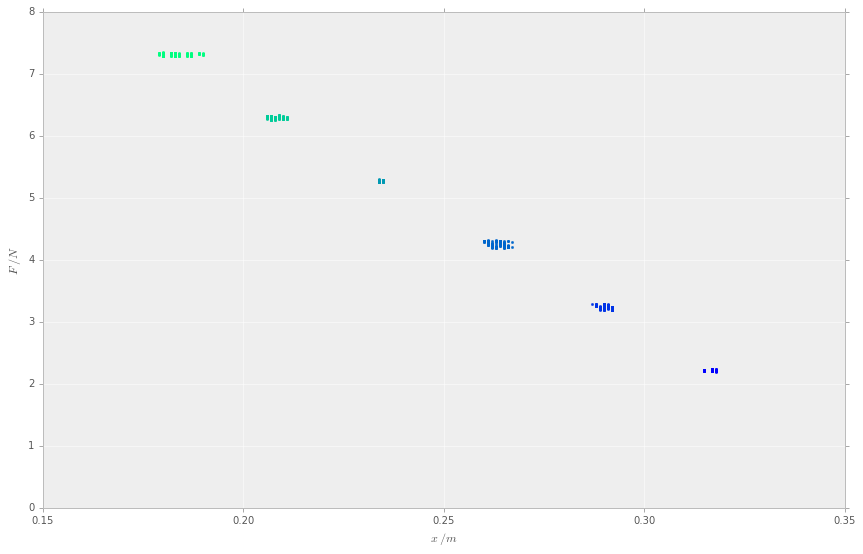
\includegraphics[max size={\textwidth}{\textheight}]{Physics IA - Data Analysis_files/Physics IA - Data Analysis_6_1.png}
    \par
    \end{center}
    
            \end{InvisibleVerbatim}
            
        
    


    % Make sure that atleast 4 lines are below the HR
    \needspace{4\baselineskip}

    
        \vspace{6pt}
        \makebox[0.1\linewidth]{\smaller\hfill\tt\color{nbframe-in-prompt}In\hspace{4pt}{[}119{]}:\hspace{4pt}}\\*
        \vspace{-2.65\baselineskip}
        \begin{ColorVerbatim}
            \vspace{-0.7\baselineskip}
            \begin{Verbatim}[commandchars=\\\{\}]
\PY{c}{\PYZsh{} Plot the x\PYZhy{}F graph with error bars.}
\PY{c}{\PYZsh{} Also, save the file with a proper name.}
\PY{n}{plt}\PY{o}{.}\PY{n}{clf}\PY{p}{(}\PY{p}{)}
\PY{n}{plt}\PY{o}{.}\PY{n}{figure}\PY{p}{(}\PY{n}{figsize}\PY{o}{=}\PY{n}{figsize}\PY{p}{(}\PY{n}{fig\PYZus{}scl}\PY{p}{)}\PY{p}{)}

\PY{n}{plt}\PY{o}{.}\PY{n}{xlim}\PY{p}{(}\PY{p}{[}\PY{l+m+mf}{0.15}\PY{p}{,} \PY{l+m+mf}{0.35}\PY{p}{]}\PY{p}{)}
\PY{n}{plt}\PY{o}{.}\PY{n}{ylim}\PY{p}{(}\PY{p}{[}\PY{l+m+mf}{0.0}\PY{p}{,} \PY{l+m+mf}{8.00}\PY{p}{]}\PY{p}{)}

\PY{n}{plt}\PY{o}{.}\PY{n}{xlabel}\PY{p}{(}\PY{l+s}{\PYZsq{}}\PY{l+s}{\PYZdl{}x}\PY{l+s}{\PYZbs{}}\PY{l+s}{; /m\PYZdl{}}\PY{l+s}{\PYZsq{}}\PY{p}{)}
\PY{n}{plt}\PY{o}{.}\PY{n}{ylabel}\PY{p}{(}\PY{l+s}{\PYZsq{}}\PY{l+s}{\PYZdl{}F}\PY{l+s}{\PYZbs{}}\PY{l+s}{; /N\PYZdl{}}\PY{l+s}{\PYZsq{}}\PY{p}{)}

\PY{n}{plt}\PY{o}{.}\PY{n}{errorbar}\PY{p}{(}\PY{p}{[}\PY{n}{x}\PY{p}{[}\PY{l+m+mi}{0}\PY{p}{]} \PY{k}{for} \PY{n}{x} \PY{o+ow}{in} \PY{n}{X}\PY{p}{]}\PY{p}{,}
             \PY{p}{[}\PY{n}{f}\PY{p}{[}\PY{l+m+mi}{0}\PY{p}{]} \PY{k}{for} \PY{n}{f} \PY{o+ow}{in} \PY{n}{F}\PY{p}{]}\PY{p}{,}
                 \PY{n}{xerr}\PY{o}{=}\PY{p}{[}\PY{n}{x}\PY{p}{[}\PY{l+m+mi}{1}\PY{p}{]} \PY{k}{for} \PY{n}{x} \PY{o+ow}{in} \PY{n}{X}\PY{p}{]}\PY{p}{,}
                 \PY{n}{yerr}\PY{o}{=}\PY{p}{[}\PY{n}{f}\PY{p}{[}\PY{l+m+mi}{1}\PY{p}{]} \PY{k}{for} \PY{n}{f} \PY{o+ow}{in} \PY{n}{F}\PY{p}{]}\PY{p}{,}
             \PY{n}{fmt}\PY{o}{=}\PY{l+s}{\PYZsq{}}\PY{l+s}{\PYZhy{}\PYZhy{}.}\PY{l+s}{\PYZsq{}}\PY{p}{,} \PY{n}{linestyle}\PY{o}{=}\PY{l+s}{\PYZdq{}}\PY{l+s}{None}\PY{l+s}{\PYZdq{}}\PY{p}{)}

\PY{n}{savefig}\PY{p}{(}\PY{l+s}{\PYZsq{}}\PY{l+s}{pt1\PYZus{}x\PYZhy{}F\PYZus{}graph}\PY{l+s}{\PYZsq{}}\PY{p}{)}
\end{Verbatim}

            
                \vspace{-0.2\baselineskip}
            
        \end{ColorVerbatim}
    

    

        % If the first block is an image, minipage the image.  Else
        % request a certain amount of space for the input text.
        \needspace{4\baselineskip}
        
        

            % Add document contents.
            
                \begin{InvisibleVerbatim}
                \vspace{-0.5\baselineskip}
\begin{alltt}<matplotlib.figure.Figure at 0x7fca0bcffd90>\end{alltt}

            \end{InvisibleVerbatim}
            
                \begin{InvisibleVerbatim}
                \vspace{-0.5\baselineskip}
    \begin{center}
    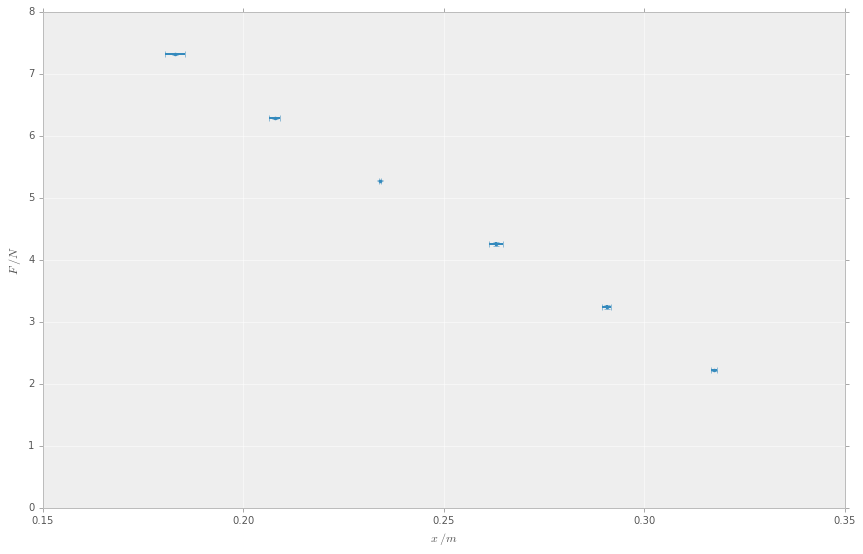
\includegraphics[max size={\textwidth}{\textheight}]{Physics IA - Data Analysis_files/Physics IA - Data Analysis_7_1.png}
    \par
    \end{center}
    
            \end{InvisibleVerbatim}
            
        
    


    % Make sure that atleast 4 lines are below the HR
    \needspace{4\baselineskip}

    
        \vspace{6pt}
        \makebox[0.1\linewidth]{\smaller\hfill\tt\color{nbframe-in-prompt}In\hspace{4pt}{[}120{]}:\hspace{4pt}}\\*
        \vspace{-2.65\baselineskip}
        \begin{ColorVerbatim}
            \vspace{-0.7\baselineskip}
            \begin{Verbatim}[commandchars=\\\{\}]
\PY{c}{\PYZsh{}\PYZsh{} Get the line of best fit for the x\PYZhy{}F graph}
\PY{n}{m}\PY{p}{,} \PY{n}{b} \PY{o}{=} \PY{n}{np}\PY{o}{.}\PY{n}{polyfit}\PY{p}{(}\PY{n}{X\PYZus{}rw}\PY{o}{.}\PY{n}{flatten}\PY{p}{(}\PY{p}{)}\PY{p}{,} \PY{n}{F\PYZus{}rw}\PY{o}{.}\PY{n}{flatten}\PY{p}{(}\PY{p}{)}\PY{p}{,} \PY{l+m+mi}{1}\PY{p}{)}

\PY{c}{\PYZsh{}\PYZsh{} Get the other bounding lines for the main line}
\PY{n}{m\PYZus{}1} \PY{o}{=} \PY{n}{get\PYZus{}slope}\PY{p}{(}\PY{p}{(}\PY{n}{X}\PY{p}{[}\PY{l+m+mi}{0}\PY{p}{]}\PY{p}{[}\PY{l+m+mi}{0}\PY{p}{]}\PY{o}{\PYZhy{}}\PY{n}{X}\PY{p}{[}\PY{l+m+mi}{0}\PY{p}{]}\PY{p}{[}\PY{l+m+mi}{1}\PY{p}{]}\PY{p}{,}
                 \PY{n}{F}\PY{p}{[}\PY{l+m+mi}{0}\PY{p}{]}\PY{p}{[}\PY{l+m+mi}{0}\PY{p}{]}\PY{o}{\PYZhy{}}\PY{n}{F}\PY{p}{[}\PY{l+m+mi}{0}\PY{p}{]}\PY{p}{[}\PY{l+m+mi}{1}\PY{p}{]}\PY{p}{)}\PY{p}{,}
                \PY{p}{(}\PY{n}{X}\PY{p}{[}\PY{o}{\PYZhy{}}\PY{l+m+mi}{1}\PY{p}{]}\PY{p}{[}\PY{l+m+mi}{0}\PY{p}{]}\PY{o}{+}\PY{n}{X}\PY{p}{[}\PY{o}{\PYZhy{}}\PY{l+m+mi}{1}\PY{p}{]}\PY{p}{[}\PY{l+m+mi}{1}\PY{p}{]}\PY{p}{,}
                 \PY{n}{F}\PY{p}{[}\PY{o}{\PYZhy{}}\PY{l+m+mi}{1}\PY{p}{]}\PY{p}{[}\PY{l+m+mi}{0}\PY{p}{]}\PY{o}{+}\PY{n}{F}\PY{p}{[}\PY{o}{\PYZhy{}}\PY{l+m+mi}{1}\PY{p}{]}\PY{p}{[}\PY{l+m+mi}{1}\PY{p}{]}\PY{p}{)}\PY{p}{)}

\PY{n}{b\PYZus{}1} \PY{o}{=} \PY{n}{get\PYZus{}intercept}\PY{p}{(}\PY{n}{m\PYZus{}1}\PY{p}{,} \PY{p}{(}\PY{n}{X}\PY{p}{[}\PY{l+m+mi}{0}\PY{p}{]}\PY{p}{[}\PY{l+m+mi}{0}\PY{p}{]}\PY{o}{\PYZhy{}}\PY{n}{X}\PY{p}{[}\PY{l+m+mi}{0}\PY{p}{]}\PY{p}{[}\PY{l+m+mi}{1}\PY{p}{]}\PY{p}{,}
                          \PY{n}{F}\PY{p}{[}\PY{l+m+mi}{0}\PY{p}{]}\PY{p}{[}\PY{l+m+mi}{0}\PY{p}{]}\PY{o}{\PYZhy{}}\PY{n}{F}\PY{p}{[}\PY{l+m+mi}{0}\PY{p}{]}\PY{p}{[}\PY{l+m+mi}{1}\PY{p}{]}\PY{p}{)}\PY{p}{)}

\PY{n}{m\PYZus{}2} \PY{o}{=} \PY{n}{get\PYZus{}slope}\PY{p}{(}\PY{p}{(}\PY{n}{X}\PY{p}{[}\PY{l+m+mi}{0}\PY{p}{]}\PY{p}{[}\PY{l+m+mi}{0}\PY{p}{]}\PY{o}{+}\PY{n}{X}\PY{p}{[}\PY{l+m+mi}{0}\PY{p}{]}\PY{p}{[}\PY{l+m+mi}{1}\PY{p}{]}\PY{p}{,}
                 \PY{n}{F}\PY{p}{[}\PY{l+m+mi}{0}\PY{p}{]}\PY{p}{[}\PY{l+m+mi}{0}\PY{p}{]}\PY{o}{+}\PY{n}{F}\PY{p}{[}\PY{l+m+mi}{0}\PY{p}{]}\PY{p}{[}\PY{l+m+mi}{1}\PY{p}{]}\PY{p}{)}\PY{p}{,}
                \PY{p}{(}\PY{n}{X}\PY{p}{[}\PY{o}{\PYZhy{}}\PY{l+m+mi}{1}\PY{p}{]}\PY{p}{[}\PY{l+m+mi}{0}\PY{p}{]}\PY{o}{\PYZhy{}}\PY{n}{X}\PY{p}{[}\PY{o}{\PYZhy{}}\PY{l+m+mi}{1}\PY{p}{]}\PY{p}{[}\PY{l+m+mi}{1}\PY{p}{]}\PY{p}{,}
                 \PY{n}{F}\PY{p}{[}\PY{o}{\PYZhy{}}\PY{l+m+mi}{1}\PY{p}{]}\PY{p}{[}\PY{l+m+mi}{0}\PY{p}{]}\PY{o}{\PYZhy{}}\PY{n}{F}\PY{p}{[}\PY{o}{\PYZhy{}}\PY{l+m+mi}{1}\PY{p}{]}\PY{p}{[}\PY{l+m+mi}{1}\PY{p}{]}\PY{p}{)}\PY{p}{)}

\PY{n}{b\PYZus{}2} \PY{o}{=} \PY{n}{get\PYZus{}intercept}\PY{p}{(}\PY{n}{m\PYZus{}2}\PY{p}{,} \PY{p}{(}\PY{n}{X}\PY{p}{[}\PY{l+m+mi}{0}\PY{p}{]}\PY{p}{[}\PY{l+m+mi}{0}\PY{p}{]}\PY{o}{+}\PY{n}{X}\PY{p}{[}\PY{l+m+mi}{0}\PY{p}{]}\PY{p}{[}\PY{l+m+mi}{1}\PY{p}{]}\PY{p}{,}
                          \PY{n}{F}\PY{p}{[}\PY{l+m+mi}{0}\PY{p}{]}\PY{p}{[}\PY{l+m+mi}{0}\PY{p}{]}\PY{o}{+}\PY{n}{F}\PY{p}{[}\PY{l+m+mi}{0}\PY{p}{]}\PY{p}{[}\PY{l+m+mi}{1}\PY{p}{]}\PY{p}{)}\PY{p}{)}

\PY{c}{\PYZsh{}\PYZsh{} Print out the values}
\PY{k}{print} \PY{l+s}{\PYZdq{}}\PY{l+s}{Line of best fit:}\PY{l+s}{\PYZdq{}}
\PY{k}{print} \PY{l+s}{\PYZdq{}}\PY{l+s}{y = \PYZob{}\PYZcb{}x + \PYZob{}\PYZcb{}}\PY{l+s}{\PYZdq{}}\PY{o}{.}\PY{n}{format}\PY{p}{(}\PY{n}{m}\PY{p}{,} \PY{n}{b}\PY{p}{)}
\PY{k}{print} \PY{l+s}{\PYZdq{}}\PY{l+s}{\PYZdq{}}
\PY{k}{print} \PY{l+s}{\PYZdq{}}\PY{l+s}{Lines of min/max slope:}\PY{l+s}{\PYZdq{}}
\PY{k}{print} \PY{l+s}{\PYZdq{}}\PY{l+s}{* y = \PYZob{}\PYZcb{}x + \PYZob{}\PYZcb{}}\PY{l+s}{\PYZdq{}}\PY{o}{.}\PY{n}{format}\PY{p}{(}\PY{n}{m\PYZus{}1}\PY{p}{,} \PY{n}{b\PYZus{}1}\PY{p}{)}
\PY{k}{print} \PY{l+s}{\PYZdq{}}\PY{l+s}{* y = \PYZob{}\PYZcb{}x + \PYZob{}\PYZcb{}}\PY{l+s}{\PYZdq{}}\PY{o}{.}\PY{n}{format}\PY{p}{(}\PY{n}{m\PYZus{}2}\PY{p}{,} \PY{n}{b\PYZus{}2}\PY{p}{)}
\end{Verbatim}

            
                \vspace{-0.2\baselineskip}
            
        \end{ColorVerbatim}
    

    

        % If the first block is an image, minipage the image.  Else
        % request a certain amount of space for the input text.
        \needspace{4\baselineskip}
        
        

            % Add document contents.
            
                \begin{InvisibleVerbatim}
                \vspace{-0.5\baselineskip}
\begin{alltt}Line of best fit:
y = -37.5365286233x + 14.1271896573

Lines of min/max slope:
* y = -39.0690034548x + 14.5782117522
* y = -36.8643692166x + 13.9526105591
\end{alltt}

            \end{InvisibleVerbatim}
            
        
    


    % Make sure that atleast 4 lines are below the HR
    \needspace{4\baselineskip}

    
        \vspace{6pt}
        \makebox[0.1\linewidth]{\smaller\hfill\tt\color{nbframe-in-prompt}In\hspace{4pt}{[}121{]}:\hspace{4pt}}\\*
        \vspace{-2.65\baselineskip}
        \begin{ColorVerbatim}
            \vspace{-0.7\baselineskip}
            \begin{Verbatim}[commandchars=\\\{\}]
\PY{c}{\PYZsh{} Plot the lines of best and worst fit.}
\PY{n}{plt}\PY{o}{.}\PY{n}{clf}\PY{p}{(}\PY{p}{)}
\PY{n}{plt}\PY{o}{.}\PY{n}{figure}\PY{p}{(}\PY{n}{figsize}\PY{o}{=}\PY{n}{figsize}\PY{p}{(}\PY{n}{fig\PYZus{}scl}\PY{p}{)}\PY{p}{)}

\PY{n}{plt}\PY{o}{.}\PY{n}{xlim}\PY{p}{(}\PY{p}{[}\PY{l+m+mf}{0.15}\PY{p}{,} \PY{l+m+mf}{0.35}\PY{p}{]}\PY{p}{)}
\PY{n}{plt}\PY{o}{.}\PY{n}{ylim}\PY{p}{(}\PY{p}{[}\PY{l+m+mf}{0.0}\PY{p}{,} \PY{l+m+mf}{8.00}\PY{p}{]}\PY{p}{)}

\PY{n}{plt}\PY{o}{.}\PY{n}{xlabel}\PY{p}{(}\PY{l+s}{\PYZsq{}}\PY{l+s}{\PYZdl{}x}\PY{l+s}{\PYZbs{}}\PY{l+s}{; /m\PYZdl{}}\PY{l+s}{\PYZsq{}}\PY{p}{)}
\PY{n}{plt}\PY{o}{.}\PY{n}{ylabel}\PY{p}{(}\PY{l+s}{\PYZsq{}}\PY{l+s}{\PYZdl{}F}\PY{l+s}{\PYZbs{}}\PY{l+s}{; /N\PYZdl{}}\PY{l+s}{\PYZsq{}}\PY{p}{)}

\PY{n}{xs} \PY{o}{=} \PY{n}{np}\PY{o}{.}\PY{n}{linspace}\PY{p}{(}\PY{l+m+mf}{0.15}\PY{p}{,} \PY{l+m+mf}{0.35}\PY{p}{,} \PY{l+m+mi}{10}\PY{p}{)}

\PY{n}{plt}\PY{o}{.}\PY{n}{plot}\PY{p}{(}\PY{n}{xs}\PY{p}{,} \PY{n}{m}\PY{o}{*}\PY{n}{xs}\PY{o}{+}\PY{n}{b}\PY{p}{,} \PY{l+s}{\PYZsq{}}\PY{l+s}{b\PYZhy{}}\PY{l+s}{\PYZsq{}}\PY{p}{,} \PY{n}{linewidth}\PY{o}{=}\PY{l+m+mi}{1}\PY{p}{)}
\PY{n}{plt}\PY{o}{.}\PY{n}{plot}\PY{p}{(}\PY{n}{xs}\PY{p}{,} \PY{n}{m\PYZus{}1}\PY{o}{*}\PY{n}{xs}\PY{o}{+}\PY{n}{b\PYZus{}1}\PY{p}{,} \PY{l+s}{\PYZsq{}}\PY{l+s}{g\PYZhy{}}\PY{l+s}{\PYZsq{}}\PY{p}{,} \PY{n}{linewidth}\PY{o}{=}\PY{l+m+mf}{0.5}\PY{p}{)}
\PY{n}{plt}\PY{o}{.}\PY{n}{plot}\PY{p}{(}\PY{n}{xs}\PY{p}{,} \PY{n}{m\PYZus{}2}\PY{o}{*}\PY{n}{xs}\PY{o}{+}\PY{n}{b\PYZus{}2}\PY{p}{,} \PY{l+s}{\PYZsq{}}\PY{l+s}{g\PYZhy{}}\PY{l+s}{\PYZsq{}}\PY{p}{,} \PY{n}{linewidth}\PY{o}{=}\PY{l+m+mf}{0.5}\PY{p}{)}

\PY{n}{plt}\PY{o}{.}\PY{n}{errorbar}\PY{p}{(}\PY{p}{[}\PY{n}{x}\PY{p}{[}\PY{l+m+mi}{0}\PY{p}{]} \PY{k}{for} \PY{n}{x} \PY{o+ow}{in} \PY{n}{X}\PY{p}{]}\PY{p}{,}
             \PY{p}{[}\PY{n}{f}\PY{p}{[}\PY{l+m+mi}{0}\PY{p}{]} \PY{k}{for} \PY{n}{f} \PY{o+ow}{in} \PY{n}{F}\PY{p}{]}\PY{p}{,}
             \PY{n}{xerr}\PY{o}{=}\PY{p}{[}\PY{n}{x}\PY{p}{[}\PY{l+m+mi}{1}\PY{p}{]} \PY{k}{for} \PY{n}{x} \PY{o+ow}{in} \PY{n}{X}\PY{p}{]}\PY{p}{,}
             \PY{n}{yerr}\PY{o}{=}\PY{p}{[}\PY{n}{f}\PY{p}{[}\PY{l+m+mi}{1}\PY{p}{]} \PY{k}{for} \PY{n}{f} \PY{o+ow}{in} \PY{n}{F}\PY{p}{]}\PY{p}{,}
             \PY{n}{fmt}\PY{o}{=}\PY{l+s}{\PYZsq{}}\PY{l+s}{r.}\PY{l+s}{\PYZsq{}}\PY{p}{,}
             \PY{n}{linestyle}\PY{o}{=}\PY{l+s}{\PYZdq{}}\PY{l+s}{None}\PY{l+s}{\PYZdq{}}\PY{p}{,}
             \PY{n}{ecolor}\PY{o}{=}\PY{l+s}{\PYZsq{}}\PY{l+s}{r}\PY{l+s}{\PYZsq{}}\PY{p}{)}

\PY{n}{savefig}\PY{p}{(}\PY{l+s}{\PYZsq{}}\PY{l+s}{pt1\PYZus{}x\PYZhy{}F\PYZus{}graph\PYZus{}fit\PYZus{}lines}\PY{l+s}{\PYZsq{}}\PY{p}{)}
\end{Verbatim}

            
                \vspace{-0.2\baselineskip}
            
        \end{ColorVerbatim}
    

    

        % If the first block is an image, minipage the image.  Else
        % request a certain amount of space for the input text.
        \needspace{4\baselineskip}
        
        

            % Add document contents.
            
                \begin{InvisibleVerbatim}
                \vspace{-0.5\baselineskip}
\begin{alltt}<matplotlib.figure.Figure at 0x7fca0bcff3d0>\end{alltt}

            \end{InvisibleVerbatim}
            
                \begin{InvisibleVerbatim}
                \vspace{-0.5\baselineskip}
    \begin{center}
    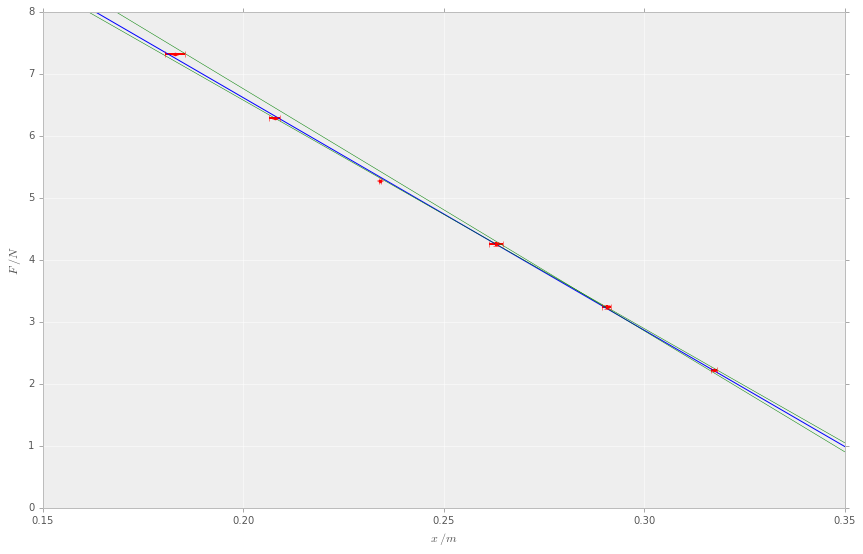
\includegraphics[max size={\textwidth}{\textheight}]{Physics IA - Data Analysis_files/Physics IA - Data Analysis_9_1.png}
    \par
    \end{center}
    
            \end{InvisibleVerbatim}
            
        
    


    % Make sure that atleast 4 lines are below the HR
    \needspace{4\baselineskip}

    
        \vspace{6pt}
        \makebox[0.1\linewidth]{\smaller\hfill\tt\color{nbframe-in-prompt}In\hspace{4pt}{[}122{]}:\hspace{4pt}}\\*
        \vspace{-2.65\baselineskip}
        \begin{ColorVerbatim}
            \vspace{-0.7\baselineskip}
            \begin{Verbatim}[commandchars=\\\{\}]
\PY{c}{\PYZsh{}\PYZsh{} Calculation of coefficient of friction and the related}
\PY{c}{\PYZsh{}\PYZsh{} uncertainties}
\PY{n}{k} \PY{o}{=} \PY{o}{\PYZhy{}}\PY{n}{m}
\PY{n}{k\PYZus{}1} \PY{o}{=} \PY{o}{\PYZhy{}}\PY{n}{m\PYZus{}1}
\PY{n}{k\PYZus{}2} \PY{o}{=} \PY{o}{\PYZhy{}}\PY{n}{m\PYZus{}2}

\PY{n}{k\PYZus{}err} \PY{o}{=} \PY{p}{(}\PY{n}{k\PYZus{}1} \PY{o}{\PYZhy{}} \PY{n}{k\PYZus{}2}\PY{p}{)}\PY{o}{/}\PY{l+m+mf}{2.0}

\PY{n}{spring\PYZus{}coeff} \PY{o}{=} \PY{n}{k}
\PY{n}{spring\PYZus{}coeff\PYZus{}err} \PY{o}{=} \PY{n}{k\PYZus{}err}

\PY{k}{print} \PY{l+s}{\PYZdq{}}\PY{l+s}{Spring coeff.}\PY{l+s}{\PYZdq{}}
\PY{k}{print} \PY{l+s}{\PYZdq{}}\PY{l+s}{Best:}\PY{l+s+se}{\PYZbs{}t}\PY{l+s}{\PYZob{}\PYZcb{} N/m}\PY{l+s}{\PYZdq{}}\PY{o}{.}\PY{n}{format}\PY{p}{(}\PY{n+nb}{round}\PY{p}{(}\PY{n}{k}\PY{p}{,} \PY{l+m+mi}{3}\PY{p}{)}\PY{p}{)}
\PY{k}{print} \PY{l+s}{\PYZdq{}}\PY{l+s}{Max:}\PY{l+s+se}{\PYZbs{}t}\PY{l+s}{\PYZob{}\PYZcb{} N/m}\PY{l+s}{\PYZdq{}}\PY{o}{.}\PY{n}{format}\PY{p}{(}\PY{n+nb}{round}\PY{p}{(}\PY{n}{k\PYZus{}1}\PY{p}{,} \PY{l+m+mi}{3}\PY{p}{)}\PY{p}{)}
\PY{k}{print} \PY{l+s}{\PYZdq{}}\PY{l+s}{Min:}\PY{l+s+se}{\PYZbs{}t}\PY{l+s}{\PYZob{}\PYZcb{} N/m}\PY{l+s}{\PYZdq{}}\PY{o}{.}\PY{n}{format}\PY{p}{(}\PY{n+nb}{round}\PY{p}{(}\PY{n}{k\PYZus{}2}\PY{p}{,} \PY{l+m+mi}{3}\PY{p}{)}\PY{p}{)}
\PY{k}{print} \PY{l+s}{\PYZdq{}}\PY{l+s}{A. Err:}\PY{l+s+se}{\PYZbs{}t}\PY{l+s}{\PYZob{}\PYZcb{} N/m}\PY{l+s}{\PYZdq{}}\PY{o}{.}\PY{n}{format}\PY{p}{(}\PY{n+nb}{round}\PY{p}{(}\PY{n}{k\PYZus{}err}\PY{p}{,} \PY{l+m+mi}{2}\PY{p}{)}\PY{p}{)}
\PY{k}{print} \PY{l+s}{\PYZdq{}}\PY{l+s}{P. Err:}\PY{l+s+se}{\PYZbs{}t}\PY{l+s}{\PYZob{}\PYZcb{}}\PY{l+s}{\PYZpc{}}\PY{l+s}{\PYZdq{}}\PY{o}{.}\PY{n}{format}\PY{p}{(}\PY{n+nb}{round}\PY{p}{(}\PY{p}{(}\PY{n}{k\PYZus{}err}\PY{o}{/}\PY{n}{k}\PY{p}{)}\PY{o}{*}\PY{l+m+mi}{100}\PY{p}{,} \PY{l+m+mi}{2}\PY{p}{)}\PY{p}{)}
\end{Verbatim}

            
                \vspace{-0.2\baselineskip}
            
        \end{ColorVerbatim}
    

    

        % If the first block is an image, minipage the image.  Else
        % request a certain amount of space for the input text.
        \needspace{4\baselineskip}
        
        

            % Add document contents.
            
                \begin{InvisibleVerbatim}
                \vspace{-0.5\baselineskip}
\begin{alltt}Spring coeff.
Best:   37.537 N/m
Max:    39.069 N/m
Min:    36.864 N/m
A. Err: 1.1 N/m
P. Err: 2.94\%
\end{alltt}

            \end{InvisibleVerbatim}
            
        
    
\section{Part 2: Calculation of Damping
coeff.}\label{part-2-calculation-of-damping-coeff.}

In a damped simple harmonic motion, the location $x$ of the particle is
given by:

$\large  x(t) = Ae^{\frac{-bt}{2m}}\cos{(\omega^\prime t + \phi)}$

Where * $A$ is the initial alplitude * $m$ is the mass of the body * $b$
is the damping coeff. *
$\displaystyle\omega^\prime = \sqrt{\omega^2 - \gamma^2} = \sqrt{\frac{k}{m} - \frac{b^2}{4m^2}}$

    % Make sure that atleast 4 lines are below the HR
    \needspace{4\baselineskip}

    
        \vspace{6pt}
        \makebox[0.1\linewidth]{\smaller\hfill\tt\color{nbframe-in-prompt}In\hspace{4pt}{[}124{]}:\hspace{4pt}}\\*
        \vspace{-2.65\baselineskip}
        \begin{ColorVerbatim}
            \vspace{-0.7\baselineskip}
            \begin{Verbatim}[commandchars=\\\{\}]
\PY{c}{\PYZsh{}\PYZsh{} Damped simple harmonic motion: EXAMPLE}
\PY{k}{def} \PY{n+nf}{ex\PYZus{}damped\PYZus{}shm}\PY{p}{(}\PY{n}{A}\PY{p}{,} \PY{n}{m}\PY{p}{,} \PY{n}{b}\PY{p}{,} \PY{n}{k}\PY{p}{,} \PY{n}{ph} \PY{o}{=} \PY{l+m+mi}{0}\PY{p}{)}\PY{p}{:}
    \PY{n}{t} \PY{o}{=} \PY{n}{np}\PY{o}{.}\PY{n}{linspace}\PY{p}{(}\PY{l+m+mi}{0}\PY{p}{,} \PY{l+m+mi}{50}\PY{p}{,} \PY{l+m+mi}{10000}\PY{p}{)}
    \PY{n}{gamma} \PY{o}{=} \PY{n+nb}{float}\PY{p}{(}\PY{n}{b}\PY{p}{)}\PY{o}{/}\PY{n+nb}{float}\PY{p}{(}\PY{l+m+mi}{2}\PY{o}{*}\PY{n}{m}\PY{p}{)}
    \PY{n}{omega} \PY{o}{=} \PY{n}{math}\PY{o}{.}\PY{n}{sqrt}\PY{p}{(}\PY{n+nb}{float}\PY{p}{(}\PY{n}{k}\PY{p}{)}\PY{o}{/}\PY{n+nb}{float}\PY{p}{(}\PY{n}{m}\PY{p}{)}\PY{p}{)}
    \PY{n}{omega\PYZus{}prime} \PY{o}{=} \PY{n}{math}\PY{o}{.}\PY{n}{sqrt}\PY{p}{(}\PY{n}{omega}\PY{o}{*}\PY{o}{*}\PY{l+m+mi}{2} \PY{o}{\PYZhy{}} \PY{n}{gamma}\PY{o}{*}\PY{o}{*}\PY{l+m+mi}{2}\PY{p}{)}
    \PY{n}{x} \PY{o}{=} \PY{p}{[}\PY{p}{]}
    \PY{k}{for} \PY{n}{T} \PY{o+ow}{in} \PY{n}{t}\PY{p}{:}
        \PY{n}{trig\PYZus{}coeff} \PY{o}{=} \PY{p}{(}\PY{n}{math}\PY{o}{.}\PY{n}{cos}\PY{p}{(}\PY{n}{omega\PYZus{}prime}\PY{o}{*}\PY{n}{T} \PY{o}{+} \PY{n}{ph}\PY{p}{)}\PY{p}{)}
        \PY{n}{exp} \PY{o}{=} \PY{p}{(}\PY{p}{(}\PY{o}{\PYZhy{}}\PY{l+m+mi}{1}\PY{o}{*}\PY{n}{T}\PY{o}{*}\PY{n+nb}{float}\PY{p}{(}\PY{n}{b}\PY{p}{)}\PY{p}{)}\PY{o}{/}\PY{n+nb}{float}\PY{p}{(}\PY{l+m+mi}{2}\PY{o}{*}\PY{n}{m}\PY{p}{)}\PY{p}{)}
        \PY{n}{x}\PY{o}{.}\PY{n}{append}\PY{p}{(}\PY{n}{A}\PY{o}{*}\PY{p}{(}\PY{n}{math}\PY{o}{.}\PY{n}{e}\PY{o}{*}\PY{o}{*}\PY{n}{exp}\PY{p}{)}\PY{o}{*}\PY{n}{trig\PYZus{}coeff}\PY{p}{)}
        
    \PY{n}{x\PYZus{}e} \PY{o}{=} \PY{n}{A}\PY{o}{*}\PY{p}{(}\PY{n}{math}\PY{o}{.}\PY{n}{e}\PY{o}{*}\PY{o}{*}\PY{p}{(}\PY{p}{(}\PY{o}{\PYZhy{}}\PY{l+m+mi}{1}\PY{o}{*}\PY{n}{t}\PY{o}{*}\PY{n+nb}{float}\PY{p}{(}\PY{n}{b}\PY{p}{)}\PY{p}{)}\PY{o}{/}\PY{n+nb}{float}\PY{p}{(}\PY{l+m+mi}{2}\PY{o}{*}\PY{n}{m}\PY{p}{)}\PY{p}{)}\PY{p}{)}
    
    \PY{n}{plt}\PY{o}{.}\PY{n}{plot}\PY{p}{(}\PY{n}{t}\PY{p}{,} \PY{n}{x}\PY{p}{,} \PY{n}{label}\PY{o}{=}\PY{l+s}{\PYZdq{}}\PY{l+s}{\PYZdl{}x(t)\PYZdl{}}\PY{l+s}{\PYZdq{}}\PY{p}{)}
    \PY{n}{plt}\PY{o}{.}\PY{n}{plot}\PY{p}{(}\PY{n}{t}\PY{p}{,} \PY{n}{x\PYZus{}e}\PY{p}{,} \PY{n}{label}\PY{o}{=}\PY{l+s}{\PYZdq{}}\PY{l+s}{\PYZdl{}x\PYZus{}b(t)\PYZdl{}}\PY{l+s}{\PYZdq{}}\PY{p}{,} \PY{n}{linewidth}\PY{o}{=}\PY{l+m+mi}{2}\PY{p}{)}
    \PY{n}{plt}\PY{o}{.}\PY{n}{legend}\PY{p}{(}\PY{p}{)}

\PY{n}{plt}\PY{o}{.}\PY{n}{clf}\PY{p}{(}\PY{p}{)}
\PY{n}{plt}\PY{o}{.}\PY{n}{figure}\PY{p}{(}\PY{n}{figsize}\PY{o}{=}\PY{n}{figsize}\PY{p}{(}\PY{n}{fig\PYZus{}scl}\PY{p}{,} \PY{n}{height\PYZus{}ratio}\PY{o}{=}\PY{p}{(}\PY{l+m+mf}{1.0}\PY{o}{/}\PY{l+m+mf}{4.0}\PY{p}{)}\PY{p}{)}\PY{p}{)}
\PY{n}{plt}\PY{o}{.}\PY{n}{xlim}\PY{p}{(}\PY{p}{[}\PY{l+m+mi}{0}\PY{p}{,} \PY{l+m+mi}{50}\PY{p}{]}\PY{p}{)}
\PY{n}{plt}\PY{o}{.}\PY{n}{xlabel}\PY{p}{(}\PY{l+s}{\PYZsq{}}\PY{l+s}{\PYZdl{}t}\PY{l+s}{\PYZbs{}}\PY{l+s}{;/s\PYZdl{}}\PY{l+s}{\PYZsq{}}\PY{p}{)}
\PY{n}{plt}\PY{o}{.}\PY{n}{ylim}\PY{p}{(}\PY{p}{[}\PY{o}{\PYZhy{}}\PY{l+m+mf}{0.45}\PY{p}{,} \PY{l+m+mf}{0.45}\PY{p}{]}\PY{p}{)}
\PY{n}{plt}\PY{o}{.}\PY{n}{ylabel}\PY{p}{(}\PY{l+s}{\PYZsq{}}\PY{l+s}{\PYZdl{}x}\PY{l+s}{\PYZbs{}}\PY{l+s}{;/m\PYZdl{}}\PY{l+s}{\PYZsq{}}\PY{p}{)}
\PY{n}{ex\PYZus{}damped\PYZus{}shm}\PY{p}{(}\PY{l+m+mf}{0.4}\PY{p}{,} \PY{l+m+mf}{0.2}\PY{p}{,} \PY{l+m+mf}{0.05}\PY{p}{,} \PY{l+m+mi}{37}\PY{p}{)}

\PY{n}{savefig}\PY{p}{(}\PY{l+s}{\PYZdq{}}\PY{l+s}{ex\PYZus{}damped}\PY{l+s}{\PYZdq{}}\PY{p}{)}
\end{Verbatim}

            
                \vspace{-0.2\baselineskip}
            
        \end{ColorVerbatim}
    

    

        % If the first block is an image, minipage the image.  Else
        % request a certain amount of space for the input text.
        \needspace{4\baselineskip}
        
        

            % Add document contents.
            
                \begin{InvisibleVerbatim}
                \vspace{-0.5\baselineskip}
\begin{alltt}<matplotlib.figure.Figure at 0x7fca0c6ef190>\end{alltt}

            \end{InvisibleVerbatim}
            
                \begin{InvisibleVerbatim}
                \vspace{-0.5\baselineskip}
    \begin{center}
    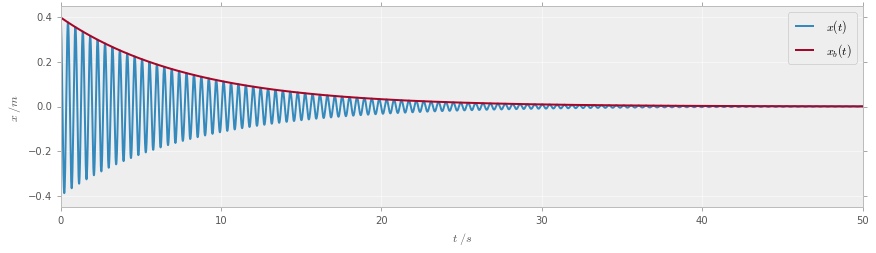
\includegraphics[max size={\textwidth}{\textheight}]{Physics IA - Data Analysis_files/Physics IA - Data Analysis_12_1.png}
    \par
    \end{center}
    
            \end{InvisibleVerbatim}
            
        
    
\subsection{Change of Phase}\label{change-of-phase}

Since all data points have different values for the phase angle, $\phi$,
for the sake of convinience, we will bring all the phases to $0$ which
will then allow us to take averages, etc.

Since the $F$ value has the most consistent readings (least number of
outliers), we shall use that to find the phase angle and then bring it
to $0$.

    % Make sure that atleast 4 lines are below the HR
    \needspace{4\baselineskip}

    
        \vspace{6pt}
        \makebox[0.1\linewidth]{\smaller\hfill\tt\color{nbframe-in-prompt}In\hspace{4pt}{[}123{]}:\hspace{4pt}}\\*
        \vspace{-2.65\baselineskip}
        \begin{ColorVerbatim}
            \vspace{-0.7\baselineskip}
            \begin{Verbatim}[commandchars=\\\{\}]

\end{Verbatim}

            
                \vspace{0.3\baselineskip}
            
        \end{ColorVerbatim}
    

        

        \renewcommand{\indexname}{Index}
        \printindex

    % End of document
    \end{document}


